\documentclass{article}
\usepackage{amsmath}
\usepackage{geometry}
\usepackage{tikz}
\usepackage{pgfplots}
\geometry{a4paper, margin=1in}
\title{Velocit\`a di un Moto Armonico}
\author{}
\date{}

\begin{document}
\maketitle

\section*{Velocit\`a di un Moto Armonico}

Dato un moto armonico di pulsazione $\omega$ e ampiezza $A$, la legge del moto \`e la seguente:
\begin{equation}
    x(t) = A \cos(\omega t)
\end{equation}

Presi due istanti separati da un tempo molto breve $t_1$ e $t_2$, l'oggetto si trover\`a in due posizioni diverse, cio\`e $x_1$ e $x_2$, e quindi lo spazio $\Delta x$ percorso nel tempo $\delta t$ sar\`a dato da:
\begin{equation}
    \Delta x = x_2 - x_1
\end{equation}

La velocit\`a all'istante $t$ \`e data dal rapporto:
\begin{equation}
    v(t) = \lim_{\delta t \to 0} \frac{\Delta x}{\delta t}
\end{equation}

Sostituendo otteniamo:
\begin{equation}
    v(t) = -A \omega \sin(\omega t)
\end{equation}

A questo punto ci servono le famigerate formule di prostaferesi, che trasformano somme e differenze di seni e coseni in prodotti. Quella che serve a noi \`e la seguente:
\begin{equation}
    \sin(a) - \sin(b) = 2 \cos\left(\frac{a + b}{2}\right) \sin\left(\frac{a - b}{2}\right)
\end{equation}

Nel nostro caso abbiamo $a = \omega t_2$ e $b = \omega t_1$, e sostituendo otteniamo:
\begin{equation}
    v(t) = -2 A \omega \cos\left(\omega t\right) \sin\left(\frac{\omega \delta t}{2}\right)
\end{equation}

Semplificando, otteniamo:
\begin{equation}
    v(t) = -A \omega \sin(\omega t)
\end{equation}

Per angoli piccoli vale con buona approssimazione $\sin(x) \approx x$, e quindi per piccoli tempi possiamo scrivere:
\begin{equation}
    v(t) \approx -A \omega \sin(\omega t)
\end{equation}

Moltiplicando e dividendo per $\delta t$, otteniamo:
\begin{equation}
    v(t) = -A \omega \sin(\omega t)
\end{equation}

A questo punto, per tempi brevi, il secondo seno e il denominatore si semplificano, e rimane solo:
\begin{equation}
    v(t) = -A \omega \sin(\omega t)
\end{equation}

Allora, per l'argomento del seno $\omega t$, arriviamo all'equazione finale:
\begin{equation}
    v(t) = -A \omega \sin(\omega t)
\end{equation}

\begin{figure}[h!]
    \centering
    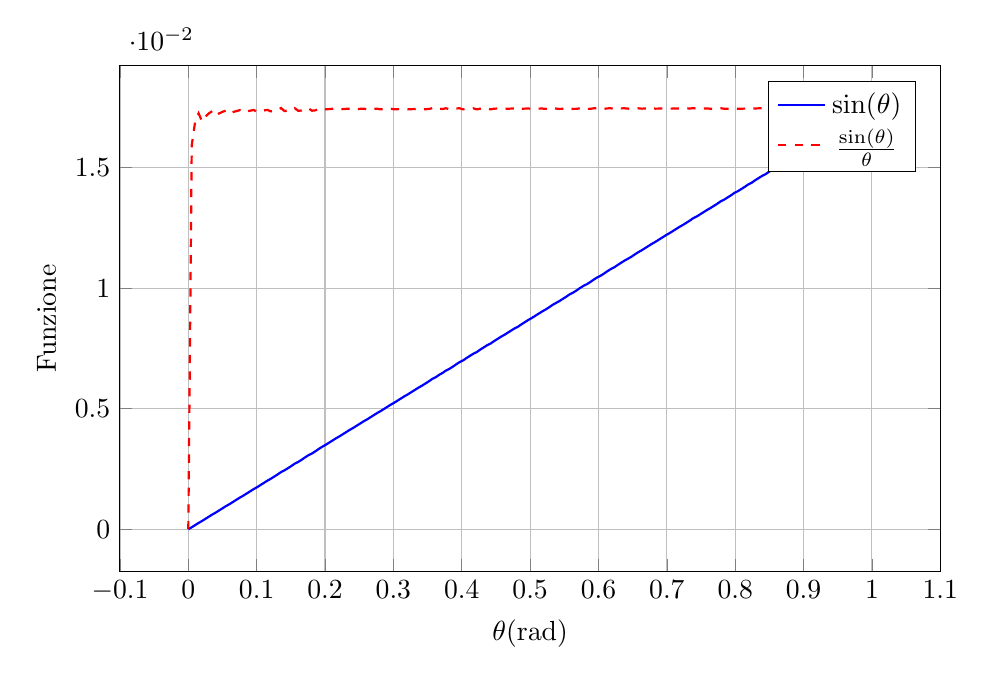
\begin{tikzpicture}
        \begin{axis}[
            xlabel={$	\theta$(rad)},
            ylabel={Funzione},
            grid=major,
            width=12cm,
            height=8cm,
            domain=0:1,
            samples=200,
            legend pos=north east
        ]
        \addplot[blue, thick] {sin(x)};
        \addlegendentry{$\sin(\theta)$}
        \addplot[red, thick, dashed] {sin(x)/x};
        \addlegendentry{$\frac{\sin(\theta)}{\theta}$}
        \end{axis}
    \end{tikzpicture}
    \caption{Grafici di $\sin(\theta)$ e $\frac{\sin(\theta)}{\theta}$ in funzione di $\theta$.}
    \label{fig:sin_div_theta}
\end{figure}

\section*{Accelerazione di un Moto Armonico}

\textbf{Compito:} Seguendo lo stesso ragionamento, ricava l'accelerazione di un moto armonico semplice.

\textbf{Aiuto:} Dovrai usare ancora una formula di prostaferesi, ma avrai differenze di seni e non coseni, e quindi quella corretta da usare \`e la seguente:
\begin{equation}
    \cos(a) - \cos(b) = -2 \sin\left(\frac{a + b}{2}\right) \sin\left(\frac{a - b}{2}\right)
\end{equation}

\end{document}
